%%%%%%%%%%%%%%%%%%%%%%%%%%%%%%%%%%%%%%%%%%%%%%%%%%%%%%%%%%%%%%%%%%%%%%%%%%%%%%%%%%
\begin{frame}[fragile]\frametitle{}

\begin{center}
{\Large Introduction to spaCy}
\end{center}
\end{frame}
%

%%%%%%%%%%%%%%%%%%%%%%%%%%%%%%%%%%%%%%%%%%%%%%%%%%%%%%%%%%%%%%%%%%%%%%%%%%%%%%%%%%
\begin{frame}[fragile]\frametitle{What is spaCy?}
  \begin{itemize}
    \item spaCy is a free, open-source library for advanced Natural Language Processing (NLP) in Python.
		\item Production ready.
		\item Used to build information extraction or natural language understanding systems, or to pre-process text for deep learning.
  \end{itemize}
	
{\tiny (Ref: https://spacy.io/usage/spacy-101)}
\end{frame}



%%%%%%%%%%%%%%%%%%%%%%%%%%%%%%%%%%%%%%%%%%%%%%%%%%%%%%%%%%%%%%%%%%%%%%%%%%%%%%%%%%
\begin{frame}[fragile]\frametitle{What spaCy isn't?}
  \begin{itemize}
    \item Not a platform or “an API” or software as a service, or a web application
		\item Not an out-of-the-box chat bot engine.
		\item Not research software.  It’s built on the latest research, but it’s designed to get things done.
		\item Not a company. It’s an open-source library. Company's name is `Explosion AI'.
  \end{itemize}
	
{\tiny (Ref: https://spacy.io/usage/spacy-101)}
\end{frame}

%%%%%%%%%%%%%%%%%%%%%%%%%%%%%%%%%%%%%%%%%%%%%%%%%%%%%%%%%%%%%%%%%%%%%%%%%%%%%%%%%%
\begin{frame}[fragile]\frametitle{Installation}
Based on OS, version, etc an installation command can be generated at https://spacy.io/usage

	
\begin{center}
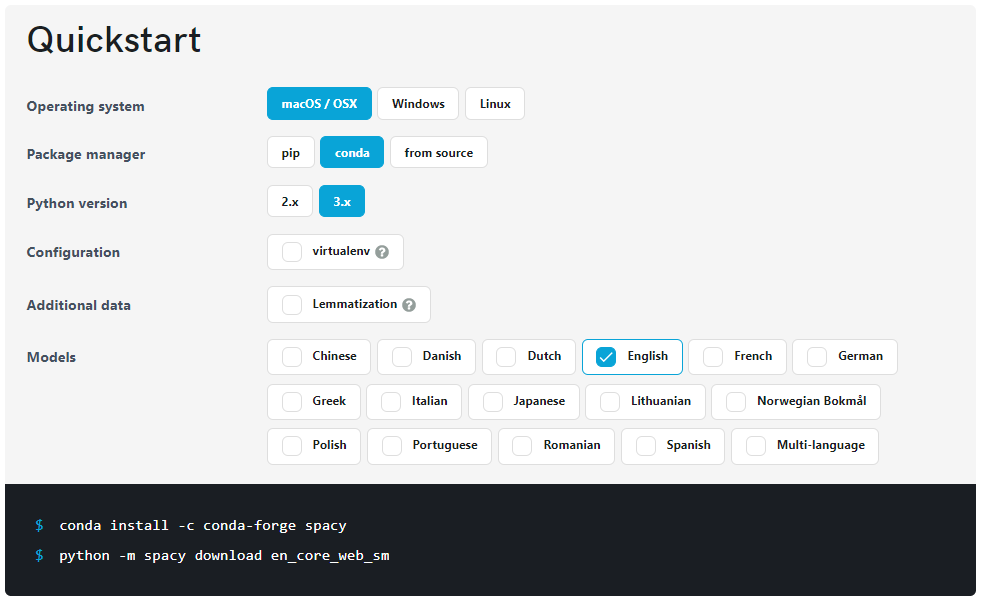
\includegraphics[width=0.8\linewidth,keepaspectratio]{spacy3}
\end{center}

{\tiny (Ref: https://spacy.io/usage/spacy-101)}
\end{frame}

%%%%%%%%%%%%%%%%%%%%%%%%%%%%%%%%%%%%%%%%%%%%%%%%%%%%%%%%%%%%%%%%%%%%%%%%%%%%%%%%%%
\begin{frame}[fragile]\frametitle{Features}
\begin{center}
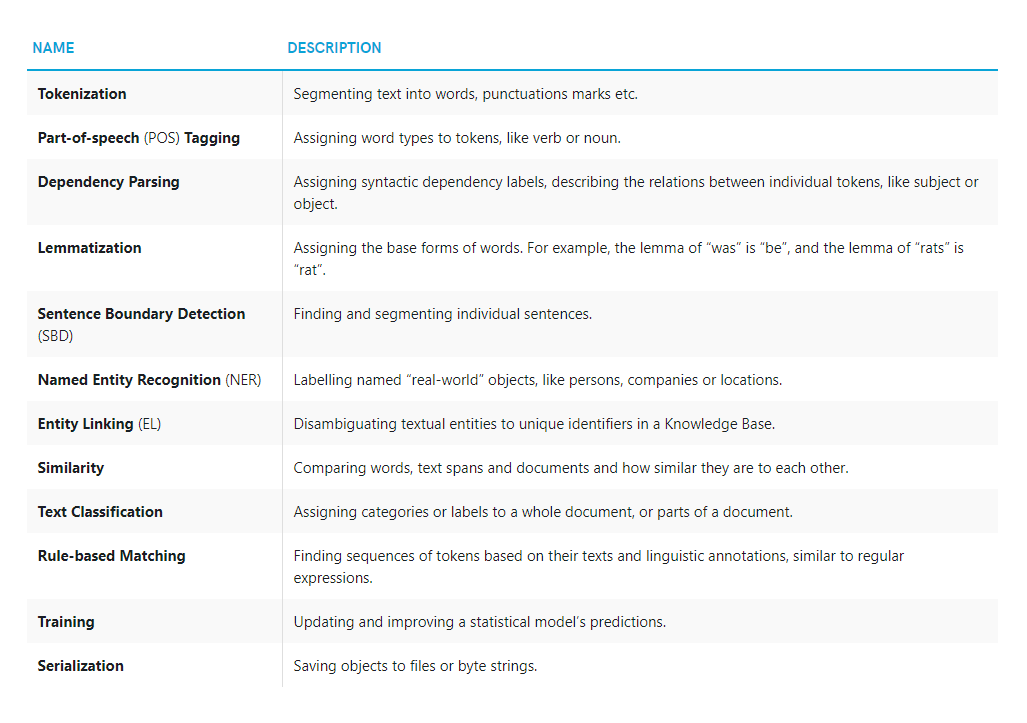
\includegraphics[width=0.8\linewidth,keepaspectratio]{spacy4}
\end{center}

{\tiny (Ref: https://spacy.io/usage/spacy-101)}
\end{frame}



%%%%%%%%%%%%%%%%%%%%%%%%%%%%%%%%%%%%%%%%%%%%%%%%%%%%%%%%%%%%%%%%%%%%%%%%%%%%%%%%%%
\begin{frame}[fragile]\frametitle{How spaCy Works?}
  \begin{itemize}
    \item Example 1: ``Apple is looking at buying U.K. startup for \$1 billion''
		\item Example 2: ``Ishu ate the Apple''
		\item `Apple' in both the above examples is different. Can spaCy identify (named entity recognition) differently?
  \end{itemize}
	
\begin{center}
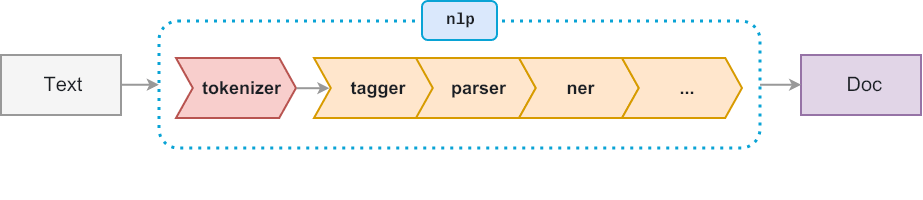
\includegraphics[width=0.8\linewidth,keepaspectratio]{spacy5}
\end{center}
	
{\tiny (Ref: https://spacy.io/usage/spacy-101)}
\end{frame}

%%%%%%%%%%%%%%%%%%%%%%%%%%%%%%%%%%%%%%%%%%%%%%%%%%%%%%%%%%%%%%%%%%%%%%%%%%%%%%%%%%
\begin{frame}[fragile]\frametitle{Pre Trained models}
\begin{itemize}
\item Pre-trained models, like 'en\_core\_web\_sm', have various NLP sub components defined. `sm' is for small.
\item Similarly other models like  'en\_core\_web\_md' (medium) and 'en\_core\_web\_lg' (large) are some of the English models.
\item Similarly `de\_core\_news\_sm' (German) and  `es\_core\_news\_sm' (Spanish) are some other language models.
\end{itemize}

\begin{center}
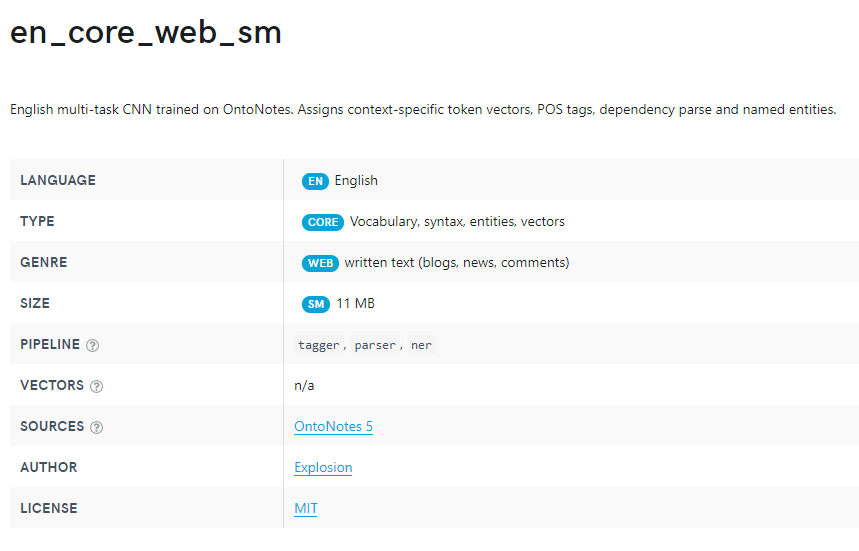
\includegraphics[width=0.6\linewidth,keepaspectratio]{spacy7}
\end{center}

\end{frame}


%%%%%%%%%%%%%%%%%%%%%%%%%%%%%%%%%%%%%%%%%%%%%%%%%%%%%%%%%%%%%%%%%%%%%%%%%%%%%%%%%%
\begin{frame}[fragile]\frametitle{Spacy Load under the hood}
  \begin{itemize}
    \item Easy to create own pipeline with reusable components.
		\item Includes spaCy’s default tagger, parser and entity recognizer, but also your own custom processing functions.
		\item At loading a model, spaCy loos at meta.json
		\begin{lstlisting}
meta.json:
{
  "lang": "en",
  "name": "core_web_sm",
  "description": "Example model for spaCy",
  "pipeline": ["tagger", "parser", "ner"]
}
\end{lstlisting}

\item Iterate over the pipeline names and create each component using \lstinline|create_pipe|, which looks them up in Language.factories
\item Add each pipeline component to the pipeline in order, using \lstinline|add_pipe|

  \end{itemize}
	
	
{\tiny (Ref: https://spacy.io/usage/spacy-101)}
\end{frame}

%%%%%%%%%%%%%%%%%%%%%%%%%%%%%%%%%%%%%%%%%%%%%%%%%%%%%%%%%%%%%%%%%%%%%%%%%%%%%%%%%%
\begin{frame}[fragile]\frametitle{Pipeline under the hood}
  \begin{itemize}
    \item When you call nlp on a text, spaCy will tokenize it and then call each component on the Doc, in order.
		\begin{lstlisting}
doc = nlp.make_doc("This is a sentence")   # create a Doc from raw text
for name, proc in nlp.pipeline:             # iterate over components in order
    doc = proc(doc)                         # apply each component

print(nlp.pipeline)
# [('tagger', <spacy.pipeline.Tagger>), ('parser', <spacy.pipeline.DependencyParser>), ('ner', <spacy.pipeline.EntityRecognizer>)]
print(nlp.pipe_names)
# ['tagger', 'parser', 'ner']
\end{lstlisting}

\item All components return the modified document, which is then processed by the component next in the pipeline.

  \end{itemize}
	
	
{\tiny (Ref: https://spacy.io/usage/spacy-101)}
\end{frame}

%%%%%%%%%%%%%%%%%%%%%%%%%%%%%%%%%%%%%%%%%%%%%%%%%%%%%%%%%%%%%%%%%%%%%%%%%%%%%%%%%%
\begin{frame}[fragile]\frametitle{Built-in pipeline components}
\begin{center}
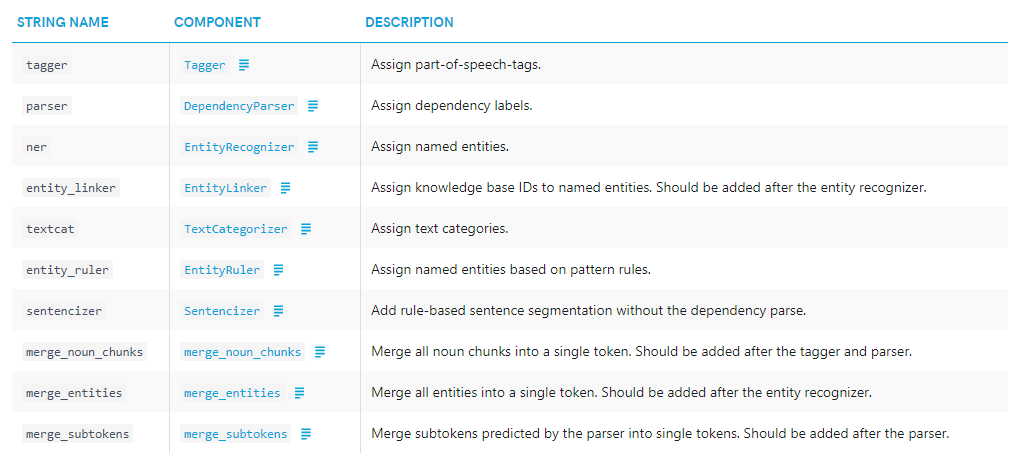
\includegraphics[width=\linewidth,keepaspectratio]{spacy10}
\end{center}

\end{frame}

%%%%%%%%%%%%%%%%%%%%%%%%%%%%%%%%%%%%%%%%%%%%%%%%%%%%%%%%%%%%%%%%%%%%%%%%%%%%%%%%%%
\begin{frame}[fragile]\frametitle{Disabling}
  \begin{itemize}
    \item If you don’t need a particular component of the pipeline – for example, the tagger or the parser, you can disable loading it
		\begin{lstlisting}
nlp = spacy.load("en_core_web_sm", disable=["tagger", "parser"])
nlp = English().from_disk("/model", disable=["ner"])
\end{lstlisting}

\item If you only need a Doc object with named entities, there’s no need to run all pipeline components on it
		\begin{lstlisting}
for doc in nlp.pipe(texts, disable=["tagger", "parser"]):
    # Do something with the doc here
\end{lstlisting}
  \end{itemize}
	
	
{\tiny (Ref: https://spacy.io/usage/spacy-101)}
\end{frame}

%%%%%%%%%%%%%%%%%%%%%%%%%%%%%%%%%%%%%%%%%%%%%%%%%%%%%%%%%%%%%%%%%%%%%%%%%%%%%%%%%%
\begin{frame}[fragile]\frametitle{Custom Component}
  \begin{itemize}
    \item A component receives a Doc object and can modify it


\item  By adding a component to the pipeline, you’ll get access to the Doc at any point during processing
  \end{itemize}
	
		\begin{lstlisting}
import spacy

def my_component(doc):
    print("After tokenization, this doc has {} tokens.".format(len(doc)))
    print("The part-of-speech tags are:", [token.pos_ for token in doc])
    if len(doc) < 10:
        print("This is a pretty short document.")
    return doc

nlp = spacy.load("en_core_web_sm")
nlp.add_pipe(my_component, name="print_info", last=True)
print(nlp.pipe_names)  # ['tagger', 'parser', 'ner', 'print_info']
doc = nlp("This is a sentence.")
\end{lstlisting}	
	
{\tiny (Ref: https://spacy.io/usage/spacy-101)}
\end{frame}

%%%%%%%%%%%%%%%%%%%%%%%%%%%%%%%%%%%%%%%%%%%%%%%%%%%%%%%%%%%%%%%%%%%%%%%%%%%%%%%%%%
\begin{frame}[fragile]\frametitle{Custom Component Class}
You can also wrap your component as a class to allow initializing it with custom settings and hold state within the component. This is useful for stateful components, especially ones which depend on shared data.
		\begin{lstlisting}
class EntityMatcher(object):
    name = "entity_matcher"
    def __init__(self, nlp, terms, label):
        patterns = [nlp.make_doc(text) for text in terms]
        self.matcher = PhraseMatcher(nlp.vocab)
        self.matcher.add(label, None, *patterns)

    def __call__(self, doc):
        matches = self.matcher(doc)
        for match_id, start, end in matches:
            span = Span(doc, start, end, label=match_id)
            doc.ents = list(doc.ents) + [span]
        return doc

nlp = spacy.load("en_core_web_sm")
terms = ("cat", "dog", "tree kangaroo", "giant sea spider")
entity_matcher = EntityMatcher(nlp, terms, "ANIMAL")

nlp.add_pipe(entity_matcher, after="ner")
\end{lstlisting}	
	
{\tiny (Ref: https://spacy.io/usage/spacy-101)}
\end{frame}